% Sección E · Evidencia, caso de negocio y recomendación.
% Figuras reducidas y texto compactado para respetar el límite de 6 páginas.

\section{Evidencia, caso de negocio y recomendación}

\paragraph{Qué muestran los datos.} Entre el 1.\textsuperscript{er} y el 2.\textsuperscript{o} semestre de 2025 el precio medio de exportación subió de 4,574 a 5,085 USD por litro (+11,2\,\%), el volumen cayó 1,5\,\% y el ingreso neto creció 9,5\,\%, de USD 26,36 a 28,85 millones: la viña facturó más vendiendo menos vino. La descomposición de la sección~4 atribuye el 108\,\% del alza a la mezcla y $-$7\,\% al precio, y entre los cuatro métodos usuales la mezcla explica entre 107 y 108\,\%. Cambió porque gran reserva pasó de 22,7\,\% a 32,5\,\% de los litros (+9,8 pp) y varietal retrocedió de 42,6\,\% a 33,3\,\% ($-$9,3 pp), mientras las listas bajaban entre 0,15\,\% y 0,19\,\% y el descuento medio subía de 3,82\,\% a 4,40\,\%, ambos ponderados por cajas.

\begin{figure}[!htbp]
  \centering
  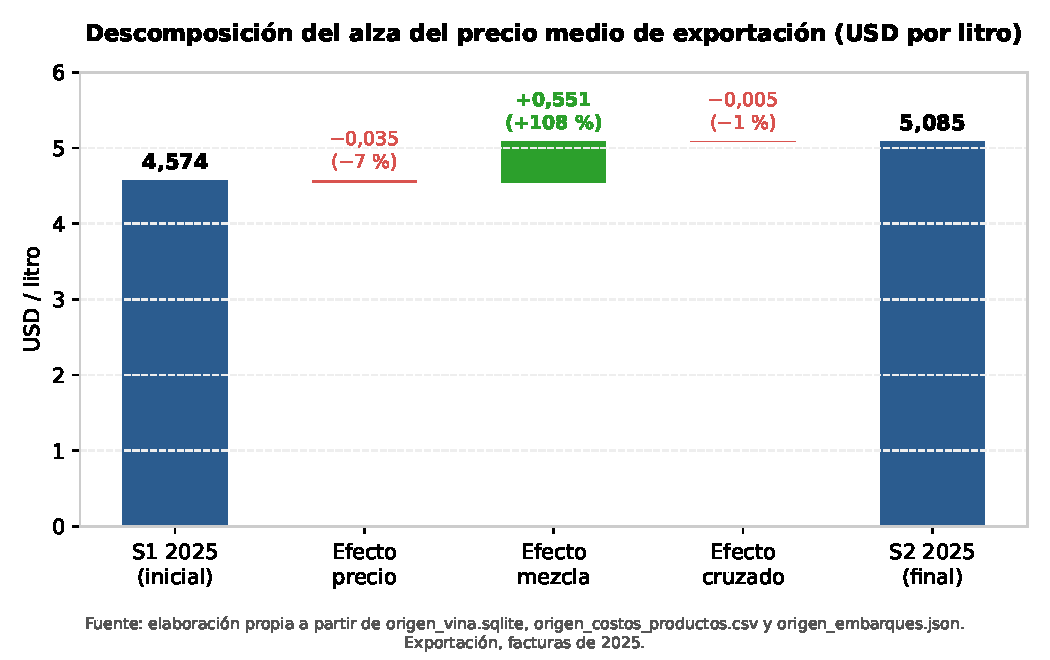
\includegraphics[width=0.44\linewidth]{figura1_cascada_precio.pdf}
  \caption{Descomposición del alza del precio medio de exportación, USD por litro. Fuente: elaboración propia sobre \texttt{fact\_venta} (10.672 líneas de exportación de 2025).}
  \label{fig:cascada}
\end{figure}

\begin{figure}[!htbp]
  \centering
  \begin{minipage}[t]{0.47\textwidth}
    \centering
    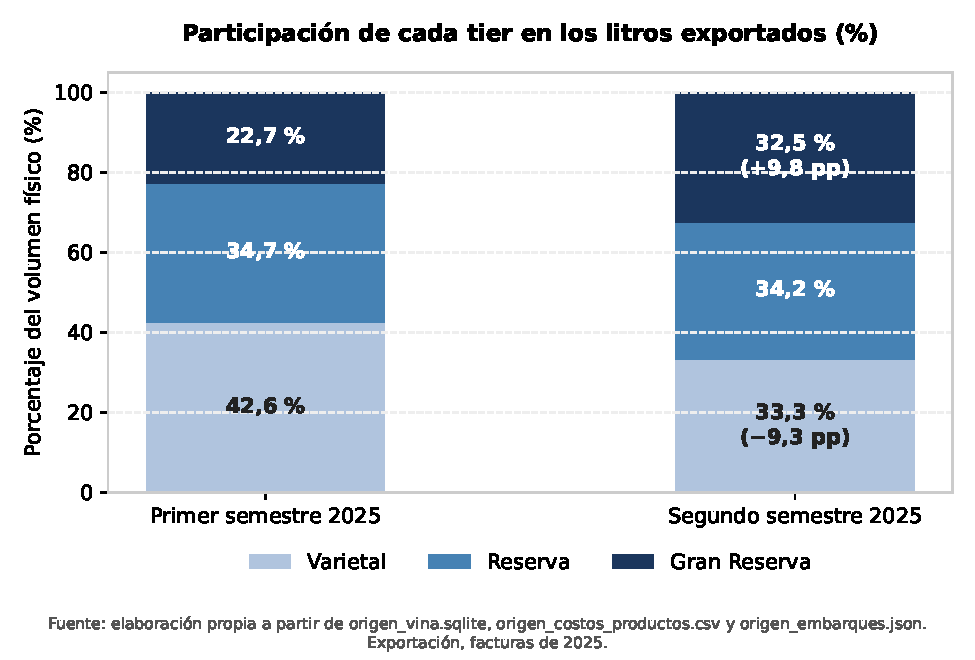
\includegraphics[width=\linewidth]{figura2_mix_semestral.pdf}
    \caption{Participación de cada tier en los litros exportados, \%. Fuente: elaboración propia sobre \texttt{fact\_venta}.}
    \label{fig:mix}
  \end{minipage}\hfill
  \begin{minipage}[t]{0.47\textwidth}
    \centering
    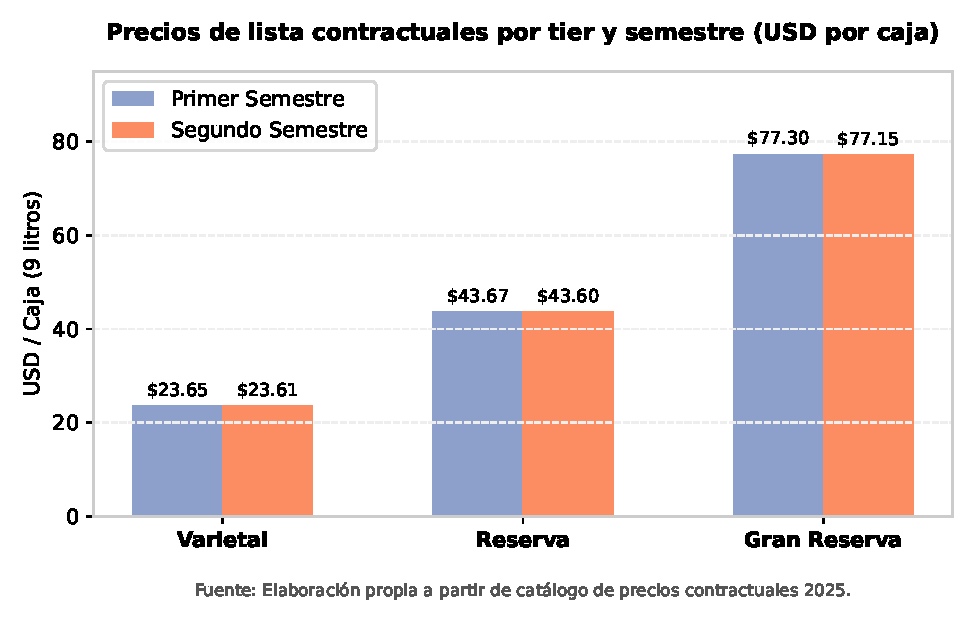
\includegraphics[width=\linewidth]{figura3_precios_lista.pdf}
    \caption{Precio de lista por caja, USD. Fuente: elaboración propia sobre \texttt{fact\_venta}.}
    \label{fig:listas}
  \end{minipage}
\end{figure}

\paragraph{Cuánto vale.} El efecto mezcla aportó 0,551 USD por litro en el 2.\textsuperscript{o} semestre: sobre sus 5.674.554 litros son \textbf{USD 3,13 millones}, o \textbf{CLP 2.961 millones} al tipo de cambio efectivo del semestre (946,34 CLP/USD). Es lo que la viña habría dejado de percibir vendiendo con la mezcla del 1.\textsuperscript{er} semestre, a los mismos precios y volumen.

\paragraph{Y nadie lo está dirigiendo.} Esos CLP 3.000 millones no vienen de una decisión comercial: «no se disgrega cepa, reserva, gran reserva ni varietal al tomar la decisión [\ldots] eso no lo tomamos como una forma de decisión en el día a día» (V). Tampoco es cosa de un cliente: los diez mercados suben entre 7,5 y 12,3 pp de gran reserva (figura~\ref{fig:mercados}, en el anexo). Y el perfil mensual no es el de una temporada: sube sostenidamente de 19,8\,\% en enero a 35,9\,\% en noviembre, y diciembre baja.

\paragraph{Recomendación.} Tres acciones, en orden de lo que cuesta hacerlas:

\begin{enumerate}
\item \textbf{Agregar dos indicadores a la planilla mensual que ya existe.} Comercial descarga el ERP a Excel una vez al mes (V); basta sumar la participación de litros de gran reserva y el precio por litro a mezcla constante. Con eso se distingue mes a mes si la facturación se movió por precio, por descuento o por mezcla, que hoy no se puede separar.
\item \textbf{Fijar la meta en mezcla, no solo en litros.} Finanzas y comercial miran litros totales y operaciones litros por cepa (V), y nadie reconcilia ambas. Una meta explícita de participación por tier alinea la asignación de uva y de bodega con lo que paga el mercado.
\item \textbf{Cerrar la definición de litros por caja en el maestro de productos.} Es una sola columna y de ella cuelga toda la medición por litro (sección~4). Mientras operaciones sostenga que las cajas no rinden lo mismo y el maestro diga 9,0 para ambos formatos, cualquier cifra por litro queda en discusión; el mismo control evita las 151 líneas cargadas este año en botellas en vez de cajas.
\end{enumerate}

\paragraph{Lo que no responde.} Con un solo año no se puede descartar del todo un componente estacional, aunque el patrón observado no es el de una temporada del hemisferio norte (bitácora, S8). El margen por mercado queda fuera: faltan costos de despacho, aranceles y la paridad dólar-euro.
